\documentclass[12pt]{article}
\usepackage{graphicx} % For inserting images
\usepackage{quantikz} % For drawing quantum circuits and dirac notation (kets)
\usepackage{enumitem} % For using letters as list numbers

\title{Quantum Computing Assignment}
\author{Nole Stites}
\date{March 2025}

\begin{document}

\maketitle

% === QUESTION 1 ===
\section{Complexity Theory Review}
Recall that, in complexity theory, PSPACE is the class of problems solvable with polynomial space but unlimited time. Considering the complexity class diagram below, why does the class PSPACE encapsulate everything?
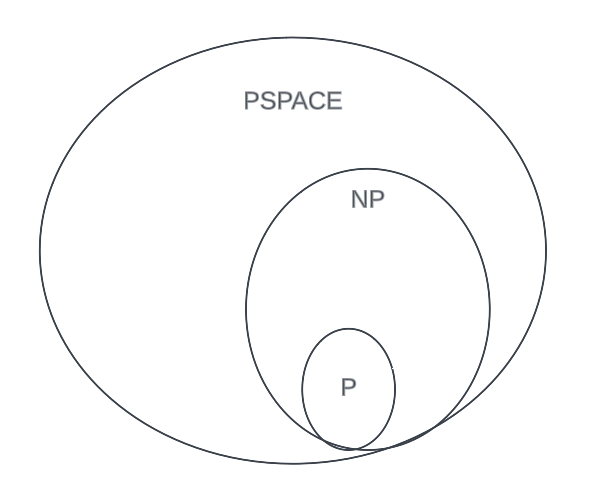
\includegraphics[]{p_np_pspace_diagram.png}

% === QUESTION 2 ===
\section{Dirac Notation}
Answer the following questions using Dirac notation. Assume that all qubits are initialized to the zero state (\ket{0}). \\
\textbf{Hint:} To verify your answers, relate them to coin flips.

\begin{enumerate}[label=\alph*)]
    \item Write the state of a one-qubit computer after applying the Hadamard gate.
    \item Write the combined state of a two-qubit computer after applying the Hadamard gate to each qubit.
    \item Write the combined state of a three-qubit computer after applying the Hadamard gate to each qubit.
\end{enumerate}

% === QUESTION 3 ===
\section{Quantum Circuit}
Use the circuit below to answer the following questions.
\[
\begin{quantikz}
\lstick{\ket{q_0}} & \gate{X} & \gate{H} & \targ{} & \qw & \qw \\
\lstick{\ket{q_1}} & \qw & \gate{H} & \ctrl{-1} & \gate{H} & \qw
\end{quantikz}
\]

\begin{enumerate}[label=\alph*)]
    \item What is the depth of the circuit?
    \item What is the space (width) of the circuit?
    \item How many total gates are there in the circuit?
    \item In Dirac notation, give the final state of the computer after the circuit has been executed. Assume that each qubit is initialized to the zero state.
\end{enumerate}

% === QUESTION 4 ===
\section{Extra Credit}
Consider the 2-qubit state
\[
\ket{\phi} = \frac{1}{\sqrt{2}}\ket{00} + \frac{1}{\sqrt{2}}\ket{11}.
\]

Show that this state is entangled by proving that there are no possible values $\alpha_0$, $\alpha_1$,
$\beta_0$, $\beta_1$ such that
\[
\ket{\phi} = (\alpha_0 \ket{0} + \alpha_1 \ket{1})(\beta_0 \ket{0} + \beta_1 \ket{1}).
\]
\textbf{Hint:} It may help to create a system of equations.
\end{document}
